\documentclass[a4paper, oneside]{book}
%Use package definitions
\usepackage[margin=1.4in]{geometry}
\usepackage[utf8]{inputenc}
%Serif font
\usepackage{cmbright}
\usepackage[T1]{fontenc}
\usepackage{textcomp}
\usepackage{amsmath, amssymb, bm}
\usepackage{pdfpages}
%Line through stuff
\usepackage{centernot}
\usepackage{transparent}
\usepackage{varwidth}
%Custom boxes
\usepackage[most]{tcolorbox}
\usepackage{xcolor}
\usepackage{url}
\usepackage{hyperref}
%Algorithm environments
\usepackage{algorithm}
\usepackage{algpseudocode}
%Header
\usepackage{titleps}

\newpagestyle{main}{
\setheadrule{.4pt}% Header rule
\sethead{MATH70027 Project 3 Solutions}{}{CID: 01859216}
% \setfootrule{.4pt}
\setfoot{}{\thepage}{}
}
\pagestyle{main}
%Space between paragraphs
\setlength{\parskip}{10pt}
%No indentation on the first word of a new paragraph
\setlength{\parindent}{0cm}
%Creating a new color box
\newtcolorbox{blackbox}[1][]{colframe=black,colback=white,sharp corners,center,#1}
%Creating the title

%Creating the title
\title{MATH70027 - Scientific Computation Project 3 Solutions\author{CID: 01859216}\date{\today}}


% -----------------------------------------------------------------------
\begin{document}
\maketitle
\section*{Part 1}
We first take a qualitative look at the different wind speeds across time, for the first 50 days.
Interestingly we see a pattern where the bright spots are flowing from left to right. 
I.e the through time we are seeing faster average daily windspeeds move in the positive
longitudinal direction, perhaps as a large storm is moving through the region from west
to east. This same pattern continues for times greater than $t=50$.

\begin{figure}[htpb]
    \centering
    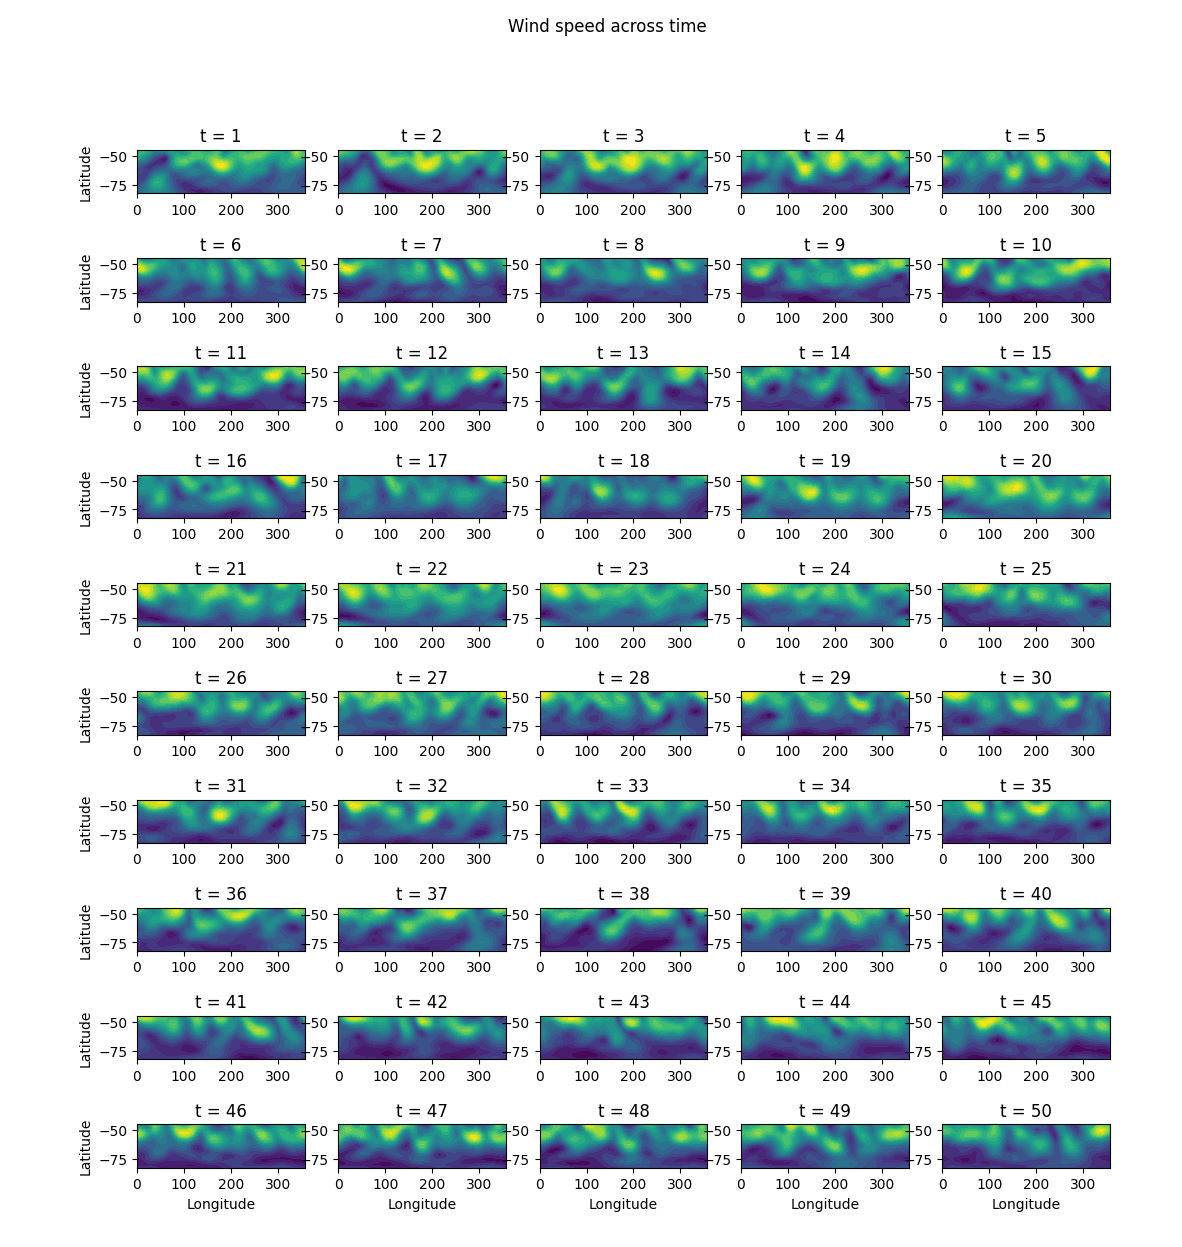
\includegraphics[width=1.0\textwidth]{./images/Pasted image 20231205152803.png}
    \caption{Wind speed for $1 \le t \le 50$}
\end{figure}

To examine the distribution of speeds through space and time we can also turn to PCA
to examine the percentage of explained variance across each of the two spacial components. I.e suppose we fix some time $t^*$ and then we denote the matrix:
$$
U := u[t^*, :, :] \in \mathbb{R}^{16 \times 144}
$$
So $U$ describes the instantaneous spacial distribution of windspeeds at some fixed time.
The rows of $U$ describe the distribution windspeeds along longitudes for some fixed latitude,
so we can apply PCA where we are considering an observation to be a row, and then
look at the explained variance of the data across each of the 144 components through time.
For times when we have most of the explained variance in the first few components, this
means that the windspeeds for different longitudes are very correlated and so the spacial distribution of windspeeds longitudinally will be very homogenous, with similar values
across fixed latitude lines. If the explained variance is more spread out across
the 144 different components then this means that the windspeeds across each
longitude line are less well correlated and the windspeeds will look different
across fixed latitude lines.

\begin{figure}[htpb]
    \centering
    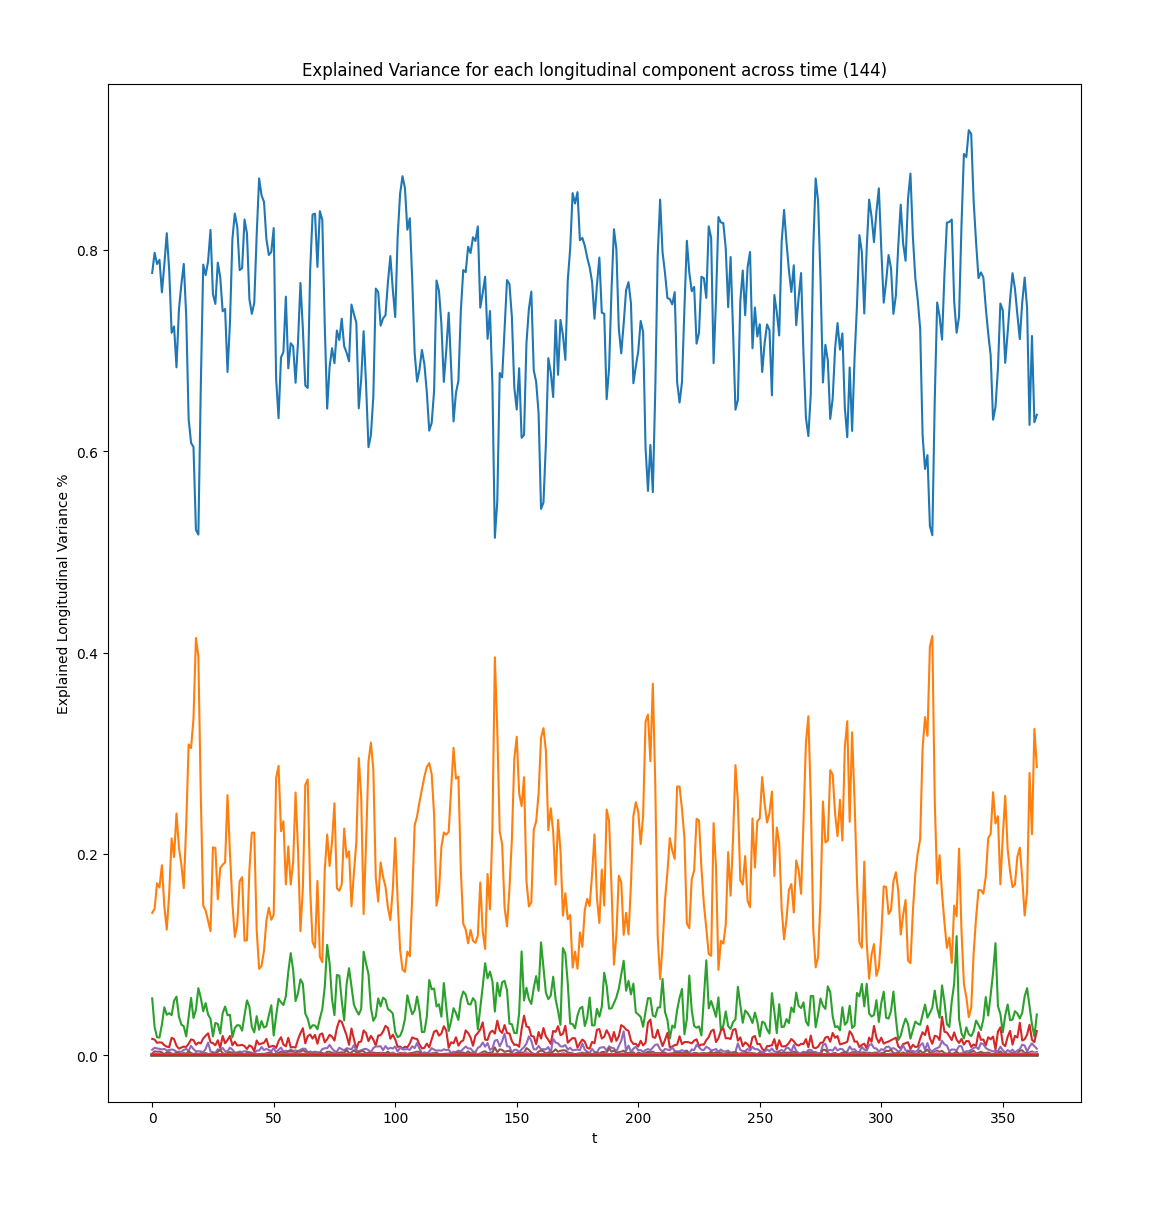
\includegraphics[width=1.0\textwidth]{./images/Pasted image 20231205164825.png}
    \caption{Explained variance for each longitudinal component. Each color represents
    the explained variance for a different principal component.}
\end{figure}


So interestingly we see at all times the majority of the explained variance is attributed
to only the first 2 out of 144 components. This clearly shows that along the lines of latitude
the windspeeds look very similar as our PCA shows that most longitudinal lines are very similar.

Then we can do the same but this time along fixed lines of longitude:

\begin{figure}[htpb]
    \centering
    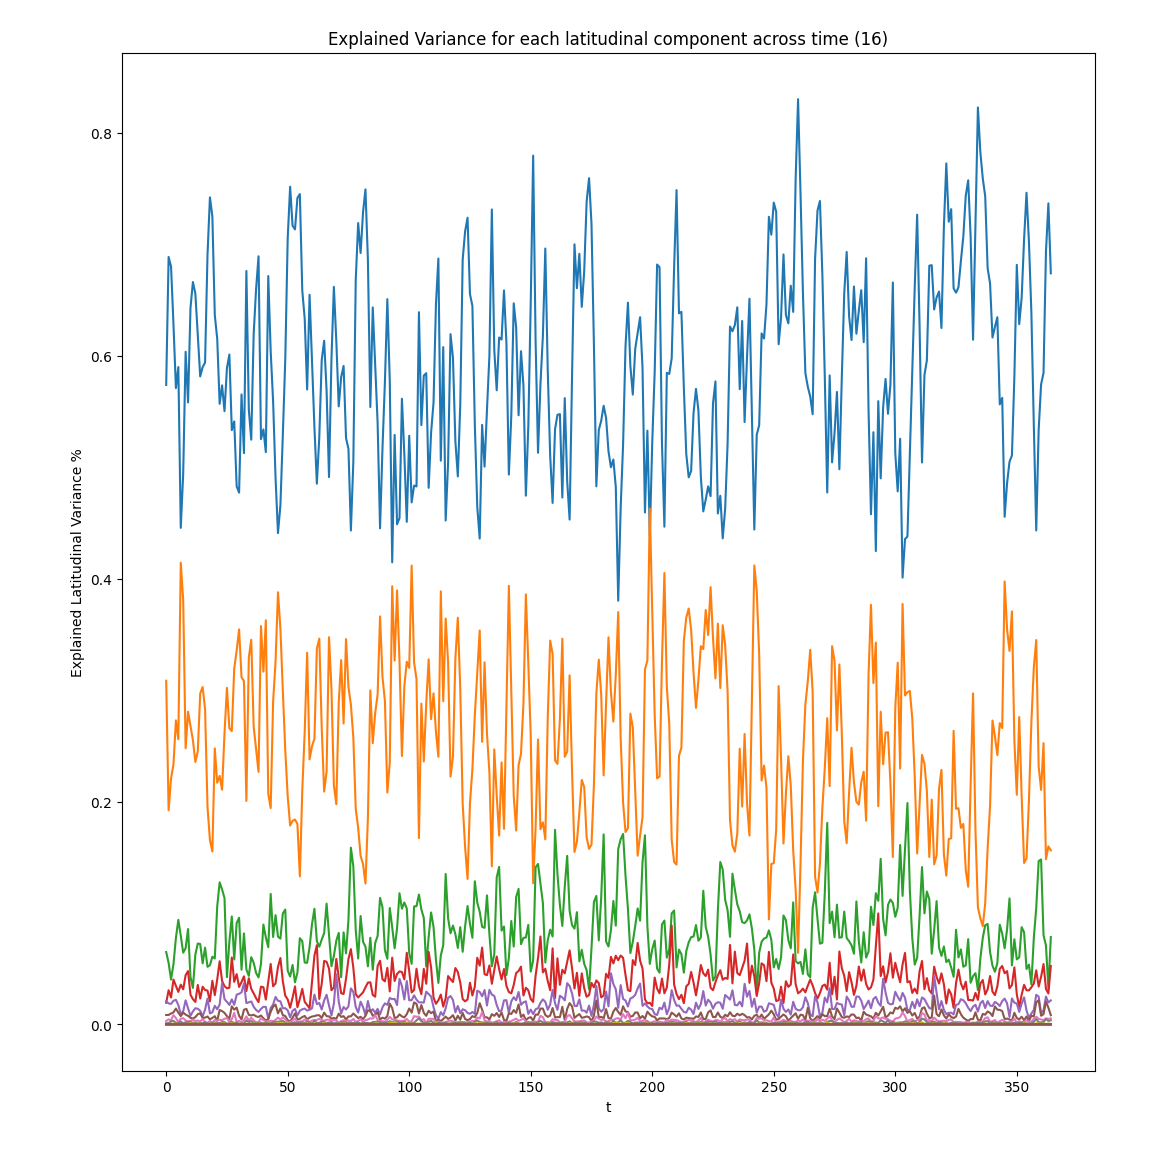
\includegraphics[width=1.0\textwidth]{./images/Pasted image 20231205164854.png}
    \caption{Explained variance for each latitudinal component. Each color represents
    the explained variance for a different principal component.}
\end{figure}

So in this case we can see that we have similar results to the longitudinal case
with most variance explained in the first few components, however this time the
difference between the first and second components explained variance is slightly less.

We see that in both these cases we fluctuate between one principal component
explaining the majority of the variance and two principal components explaining
the majority of the variance. We can interpret this as the windspeeds 
moving from very homogenous spacial distributions, with most windspeeds
similar in most regions, to a distributions with two main windspeed types,
i.e high and low.
This supports our qualitative findings above, where we found that we seem to
move from configurations with relatively evenly distributed wind speeds,
to configurations with concentrated areas of high wind speeds.
\clearpage

So we have used PCA to examine the fluctuations through space for fixed times, and now we will
use PCA to examine the fluctuations through time for fixed space.
We do this by flattening the 3D $u$ array into a 2D array and then taking the transpose,
so we columns which represent times and rows which represent a flattened version of $u[t, :, :]$. 
Then when we take the PCA of this array and plot the first few principal components with
the most explained variance, we are visualizing the dominant spatial pattern of variability of windspeeds through time.


So we first plot the cumulative explained variances for the first $n$ principal
components, where we vary $n$. 
\begin{figure}[htpb]
    \centering
    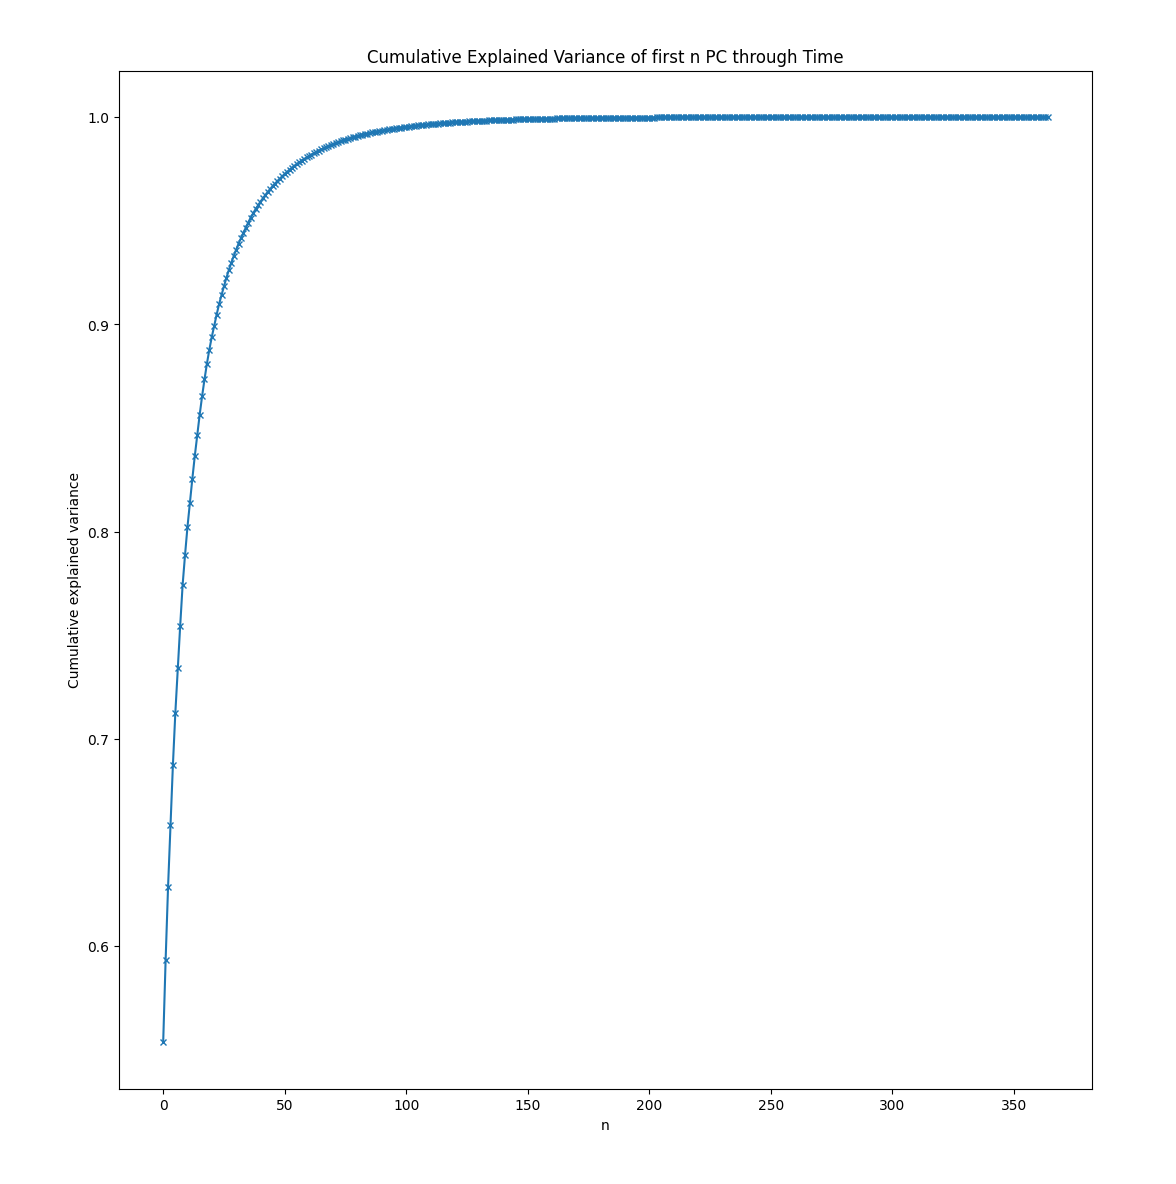
\includegraphics[width=1.0\textwidth]{./images/explained_var_through_time.png}
    \caption{Cumulative explained variance through time.}
\end{figure}

So interestingly we see that we can explain
almost all of our variance with the first approx 100 principal components.
We plot these first 100 principal components below.


\begin{figure}[htpb]
    \centering
    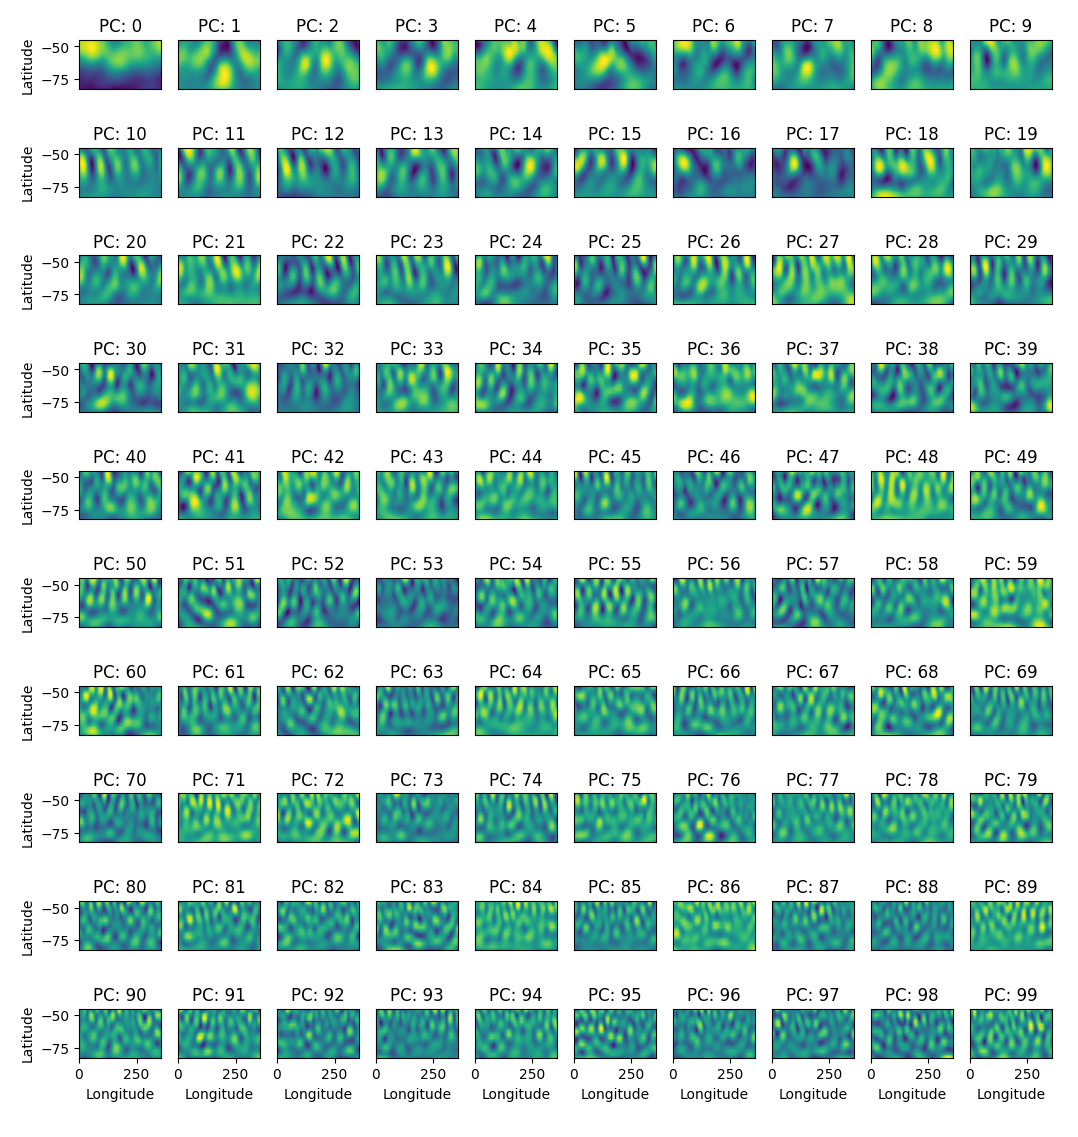
\includegraphics[width=1.0\textwidth]{./images/first_81_pc_through_time.png}
    \caption{First 100 principal components through time.}
\end{figure}

The bright areas of our plotted principal components show us the regions of latitude and longitude
where the windspeed varies the most, and the darker areas show us where the windspeed varies the least.
If we look at the first principal component, we can see that around 50\% of the windspeed
variation happens in the most northern latitudes. We also see from the 2nd principal component
that we have also a very bright region at around (-75, 150) which is the (latitude, longitude) of Antarctica,
which is a very cold and windy place, so it makes sense that we would also have a lot of variation in windspeeds here.

Then for the other principal components we see that we have mostly noise with a much smaller
explained variance.


\clearpage


We can also look at the 2D fourier transform of the windspeed through space.
We calculate the Fourier Transform of the 2D image, $u[t, :, :]$ for each $t$ and then
sum over $t$. (We also take logs to make the different levels more visible).

\begin{figure}[htpb]
    \centering
    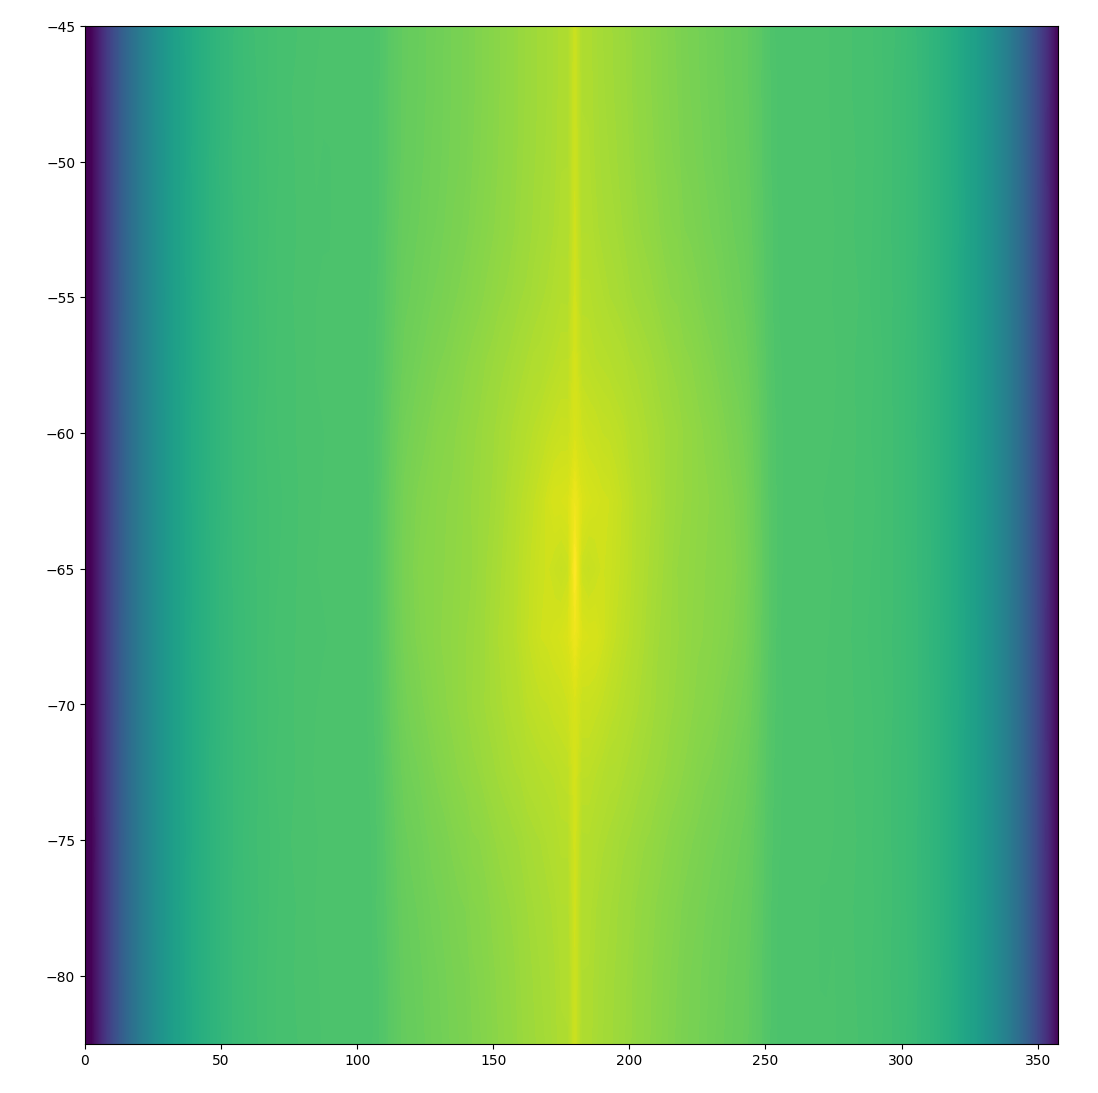
\includegraphics[width=0.7\textwidth]{./images/Pasted image 20231206105122.png}
    \caption{Sum of fourier spectra of wind speeds across all times.}
\end{figure}

Clearly we see distinct vertical lines, indicating periodic vertical spatial structure.
This shows that the windspeeds are oscillating periodically from north to south,
and south to north.


\section*{Part 2}
\subsection*{Part 2.1}
We implement method 2 by noticing that the system can be written in terms of matrices.
If we denote by $\tilde{f} \in \mathbb{R}^{m-1 \times n}$ the matrix whose $(i,j){th}$ element is $\tilde{f}_{i,j}$ and similarly for $f \in \mathbb{R}^{m \times n}$.
If we also define: 
$$
A := \begin{pmatrix}
1 & 0 & 0 & 0 & 0 & \dots & 0 & 0 & 0 \\
\alpha & 1 & \alpha & 0 & 0 & \dots & 0 & 0 & 0 \\
0 & \alpha & 1 & \alpha & 0 & \dots & 0 & 0 & 0 \\
0 & 0 & \alpha & 1 & \alpha & \dots & 0 & 0 & 0 \\
\vdots & \vdots & \vdots & \vdots & \vdots & \dots & \vdots & \vdots & \vdots \\
0 & 0 & 0 & 0 & 0 & \dots & \alpha & 1 & \alpha \\
0 & 0 & 0 & 0 & 0 & \dots & 0 & 0 & 1
\end{pmatrix} \in \mathbb{R}^{m-1 \times m-1}
$$
$$
B := \begin{pmatrix}
\tilde{a} & \tilde{b} & \tilde{c}  & \tilde{d}  & 0 & \dots & 0 &  0 & 0 & 0 \\
\frac{b}{2} & \frac{a}{2} & \frac{a}{2} & \frac{b}{2} & 0 & \dots & 0 & 0 & 0 & 0 \\
0 & \frac{b}{2} & \frac{a}{2} & \frac{a}{2} & \frac{b}{2} & \dots & 0 & 0 & 0 & 0 \\
0 & 0 & \frac{b}{2} & \frac{a}{2} & \frac{a}{2}  & \dots & 0 & 0 & 0 & 0 \\
\vdots  & \vdots & \vdots  & \vdots  & \vdots  & \dots & \vdots  & \vdots  & \vdots & \vdots \\
0 & 0 & 0 & 0 & 0 & \dots & \frac{b}{2} & \frac{a}{2} & \frac{a}{2} & \frac{b}{2} \\
0 & 0 & 0 & 0 & 0 & \dots & \tilde{a} & \tilde{b} & \tilde{c} & \tilde{d}
\end{pmatrix} \in \mathbb{R}^{m-1 \times m}
$$

Then we can write:  $A \tilde{f} = B f$  which is linear system which we solve.
Note that $A$ is a banded matrix, with 1 lower diagonal and 1 upper diagonal,
so we can take advantage of this structure and use the scipy.linalg.solve\_banded
method.

\subsection*{Part 2.2}
Firstly we analyse the theoretical computational cost of both methods.
In method 1 we are adding two $m-1 \times n$ matrices and so we have $(m-1)n$ additions
and so method 1 has time complexity $O(mn)$.

For method 2, firstly we have to construct the matrix $ab$ and $B$. 
Note: since we are using Scipy's linalg solve\_banded method we don't have to 
construct the full $A$ matrix, instead we just construct $ab \in \mathbb{R}^{3 \times m-1}$ which consists
of the upper, main and lower diagonals of $A$ stacked together.
The time complexity of these constructions is clearly $O(m)$.

Then we have to compute the matrix multiplication $Bf \in \mathbb{R}^{m-1 \times n}$. Since $B$ is mostly sparse, with only $4$  non-zero elements per row, we can use sparse matrices and then we will only have 4 multiplications and 3 additions to calculate $[Bf]_{i,j}$ and so the multiplication $Bf$  has
time complexity $O(mn)$. Then after the constructions we call scipy.linalg.solve\_banded which uses the LAPACK gtsv routine, since we only have 1 upper and 1 lower diagonal i.e $A$ is tridiagonal.
This routine runs in $O(N)$ time for $N \times N$ matrices when we $1$ system of equations. i.e when $A \mathbf{x} = \mathbf{b}$ where $\mathbf{b}$ is a vector. So if instead we have $A X = B$ where $B$ is a matrix, this is calculated by running the routine for each column of $B$, and so if $A \in \mathbb{R}^{m-1 \times m-1}$ and $B \in \mathbb{R}^{m-1 \times m}$ it follows that we have time complexity $O(m^{2})$.
So overall our time complexity is $O(mn + m^{2})$. If we consider $n$ to be of the same magnitude as $m$ then both method 1 and method 2 have the same theoretical asymptotic time complexity.

Now we look to some experimental results to verify our theoretical results.

We can look at the wall time for increasing values of $m$ for each method.

\begin{figure}[htpb]
    \centering
    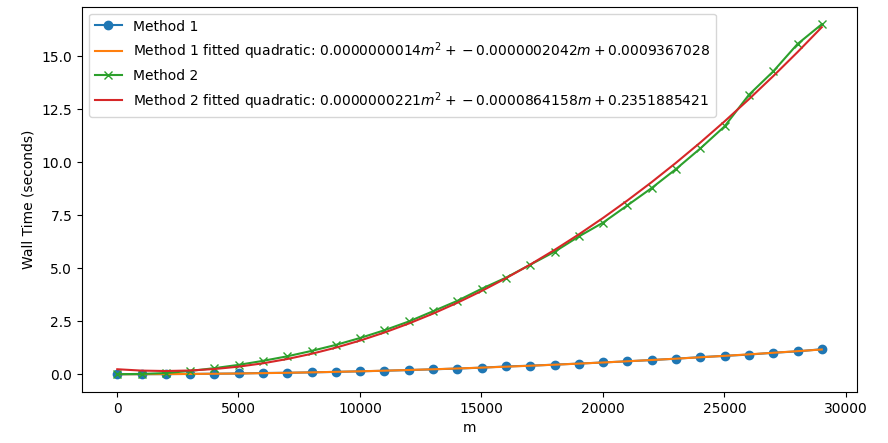
\includegraphics[width=1.0\textwidth]{./images/Screenshot_2023-12-08_13-34-06.png}
    \caption{Wall times as a function of $m$ for method 1 and method 2.}
\end{figure}

\begin{figure}[htpb]
    \centering
    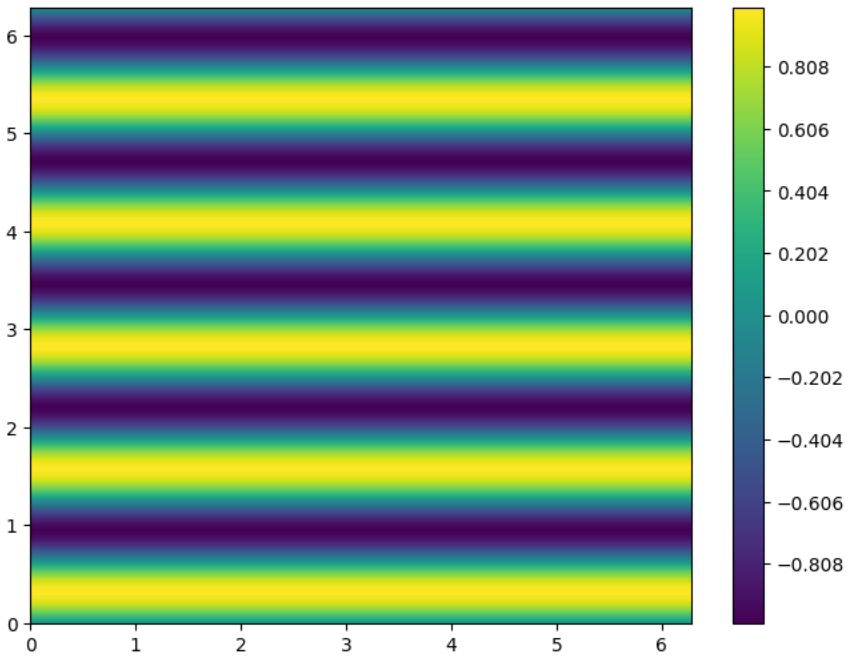
\includegraphics[width=1.0\textwidth]{./images/sin_k5.png}
    \caption{$f = \sin(ky)$ for wavenumber $k = 5$.}
\end{figure}

(We have set $n = m$ since it is given that $n$ and $m$ are of the same magnitude). So clearly we
observe quadratic behaviour in $m$, for both, just as we had predicted. Although the coefficient for method 1 is clearly much smaller than for method 2 and we see
that the wall times for method 1 are much smaller than for method 2. This makes
sense since method 1 is much simpler and is using vectorized numpy addition, which
uses concurrency to parallelize operations.


So next we examine the accuracy of both methods.
We first look at the accuracy when interpolating the $\sin$ function with wavenumber $k$.
(See below figure for example, with $k = 5$).

\clearpage

We vary the wavenumber, $k$, and calculate the difference between the ground truth, $f_I := \sin(ky_I)$ 
and the predicted $\tilde{f_I} = \text{part2}(f)$ for both method 1 and method 2 and then
compare the MSE of the results compared to the ground truth. 

\begin{figure}[htpb]
    \centering
    \includegraphics[width=1.0\textwidth]{./images/wavenumber\_mse.png}
    \caption{MSE of interpolated results compared to ground truth for method 1 and 2.}
\end{figure}

So interestingly we see that for lower wavenumbers, method 1 performs best, perhaps
since lower wave numbers means smaller gradients/less steep changes in slope. Then once
we go past around $k=500$ method 2 gives better results (in terms of MSE), again perhaps because
method 2 is analagous to the implicit finite differences method of differentiation and
method 1 is analagous to 2nd order finite differences method and in lectures we saw that
the implicit method performs better than 2nd order method for higher wave numbers. So
if we have a better approximator of the derivative, it makes sense that we would
also be able to interpolate better for higher wavenumbers because interpolation and differentation
are analagous methods.

In order to examine this further we do some wavenumber analysis using $f(x) = e^{ikx}$.
Firstly we start off with calculating the wavenumber for method 1:

\begin{align}
e^{ikx} &= \frac{1}{2}(e^{ik(x+1/2h)} + e^{ik ( x - 1/2h)}) \\
&= \frac{1}{2} e^{ikx} [e^{ikh/2} + e^{-ikh/2}] \\
&= e^{ikx}[\cos(kh/2)]
\end{align}

So the key question is how close is $\cos(kh / 2)$ to $1$.
When $kh \neq  0$ this is equivalent to asking how close is $kh$ to  $kh \cos(kh / 2)$. So this gives us:
\[
kh' = kh \cos(kh / 2)
.\]

Then for method 2 analagously we do:
$$
\alpha e^{ik(x -h)} + e^{ikx} + \alpha e^{ik(x+h)} = \left[ \frac{b}{2} (e^{ik(x+3/2 h)} + e^{ik(x-3/2h)})  + \frac{a}{2}(e^{ik(x + 1/2h)} + e^{ik(x-1/2h)})\right]
$$
And then we can pull out the $e^{ikx}$ term from both sides and we get:
$$
\alpha e^{-ikh} + 1 + \alpha e^{ikh} = \frac{b}{2}(e^{3/2ikh} + e^{-3/2ikh}) + \frac{a}{2}(e^{1/2ikh} + e^{-1/2ikh})
$$
And so simplifying this we get:
$$
1 = b\cos\left( \frac{3}{2}kh \right) + a\cos\left( \frac{1}{2}kh \right) - 2\alpha \cos(kh)
$$
And so can multiply both sides by $kh$ and then the LHS to get:
$$
kh' = kh \left(b\cos\left( \frac{3}{2}kh \right) + a\cos\left( \frac{1}{2}kh \right) - 2\alpha \cos(kh)\right)
$$
We can then plot the calculated $kh'$ values:

\begin{figure}[htpb]
    \centering
    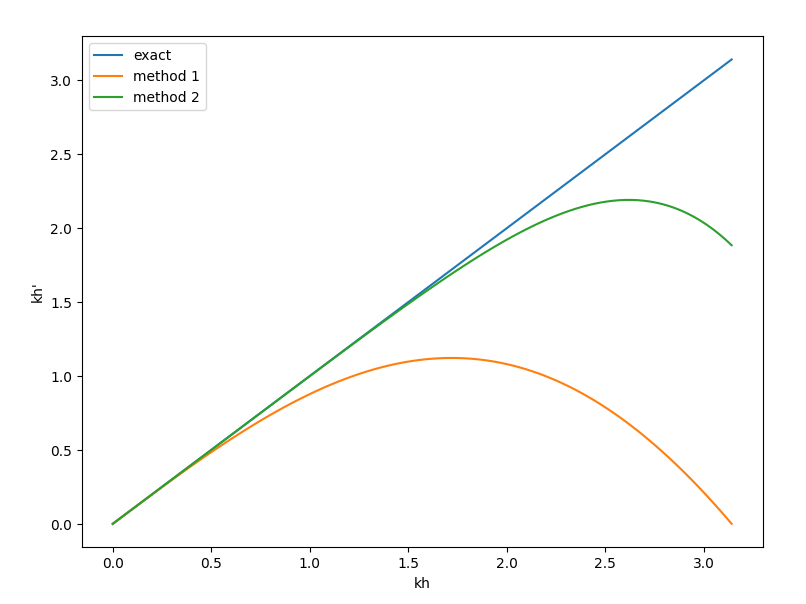
\includegraphics[width=0.7\textwidth]{./images/wavenumber_analysis.png}
    \caption{Wavenumber analysis comparing method 1 to method 2.}
\end{figure}

This clearly shows further that for higher wavenumbers method 2 is a better choice
and is a better interpolator.

We can calculate the error by finding the $kh^*$ such that:
\[
\frac{kh^* - kh'}{kh^*} \approx 0.01
.\]
I.e the $kh$ that gives us a $1\%$ relative interpolation error.

So for method 1 we find that $kh^* \approx 0.28$ and for method 2 we find  $kh^* \approx 1.57$.

Then we can use the fact that $\lambda = 2\pi / k$ and to get for method 1 we have
$2\pi / 0.28 \approx 22$ points per wavelength and for method 2 we have $2\pi / 1.57 \approx 4$ points
per wavelength for a $\approx 1\%$ error. So this means when we have fewer data points
for some fixed area, we should use method 2 for interpolation over method 1,
but when we have more/denser data, we should use method 1.


Also if computational performance (e.g wall times) is a constraint,
then method 1 should be chosen.





\section*{Part 3}
We start off by plotting the solutions for $u_{i}$ with $100 \leq i \leq n - 100$ for $n := 4000$ 
for different values of $c \in [0.5, 1.5]$. We see in the below figures that for $c$ from $0.5$ to $0.9$
we observe stable steady sinusoidal oscillations in time, with uniform values for all $u_{i}$ for each fixed
time. As time progresses the solution oscillates regularly between low and high values.
For $c=0.5$ we see the regular oscillations have the lowest frequency and as we increase
$c$ the frequency of these oscillations increases. Then as we move from $c > 0.9$ we see
instabilities occuring, with some chaotic behaviour. At $c=1.1$ we still observe
fairly regular behaviour but with some perturbations from the regular oscillations
towards the final times. Then from $c=1.3$ onwards we observe much larger
perturbations with increased chaotic behaviour.


\begin{figure}[htpb]
    \centering
    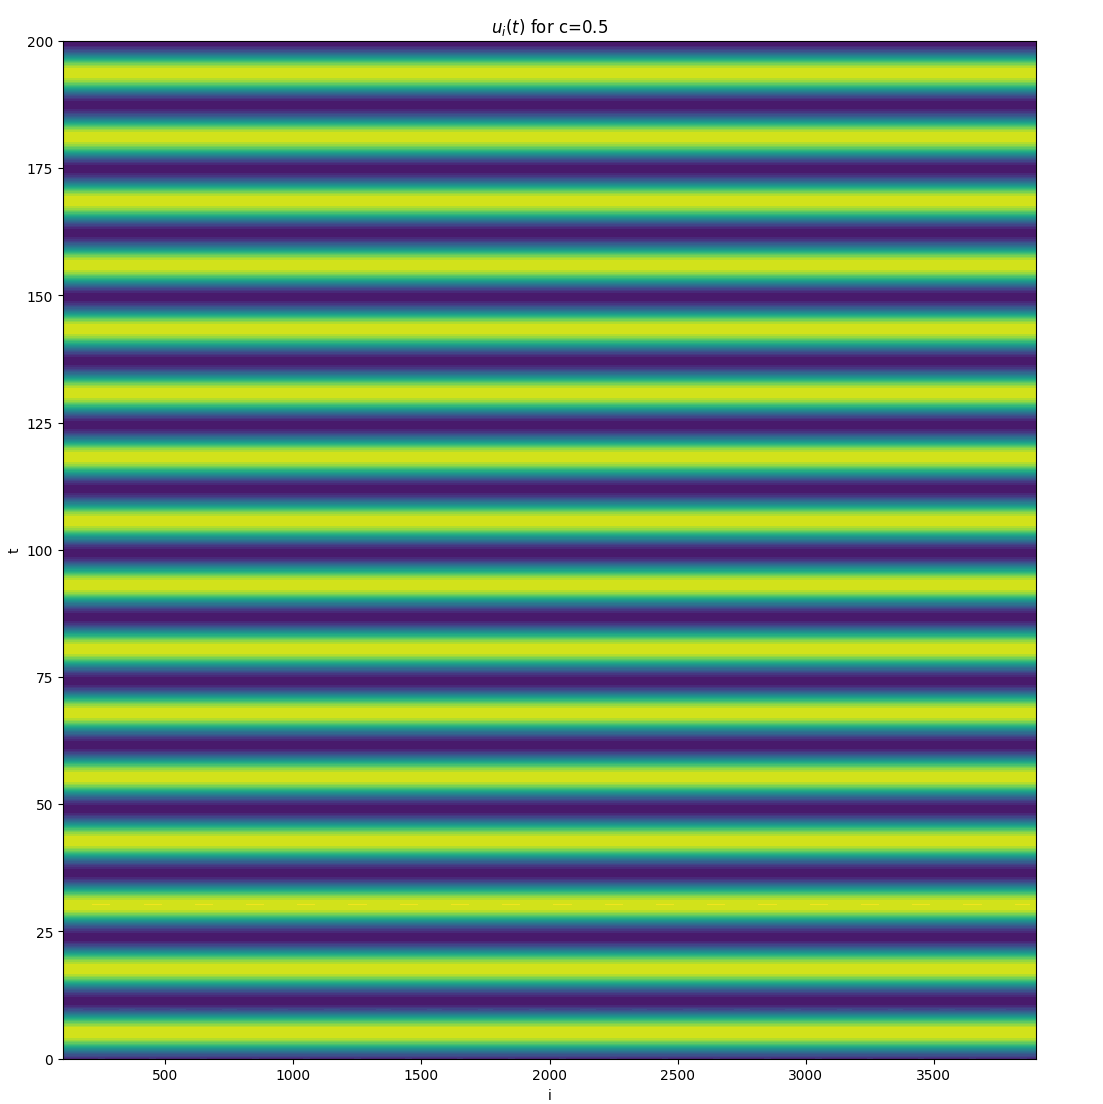
\includegraphics[width=1.0\textwidth]{./images/Pasted image 20231207115743.png}
    \caption{$u_i(t)$ for $c=0.5$}
\end{figure}

\begin{figure}[htpb]
    \centering
    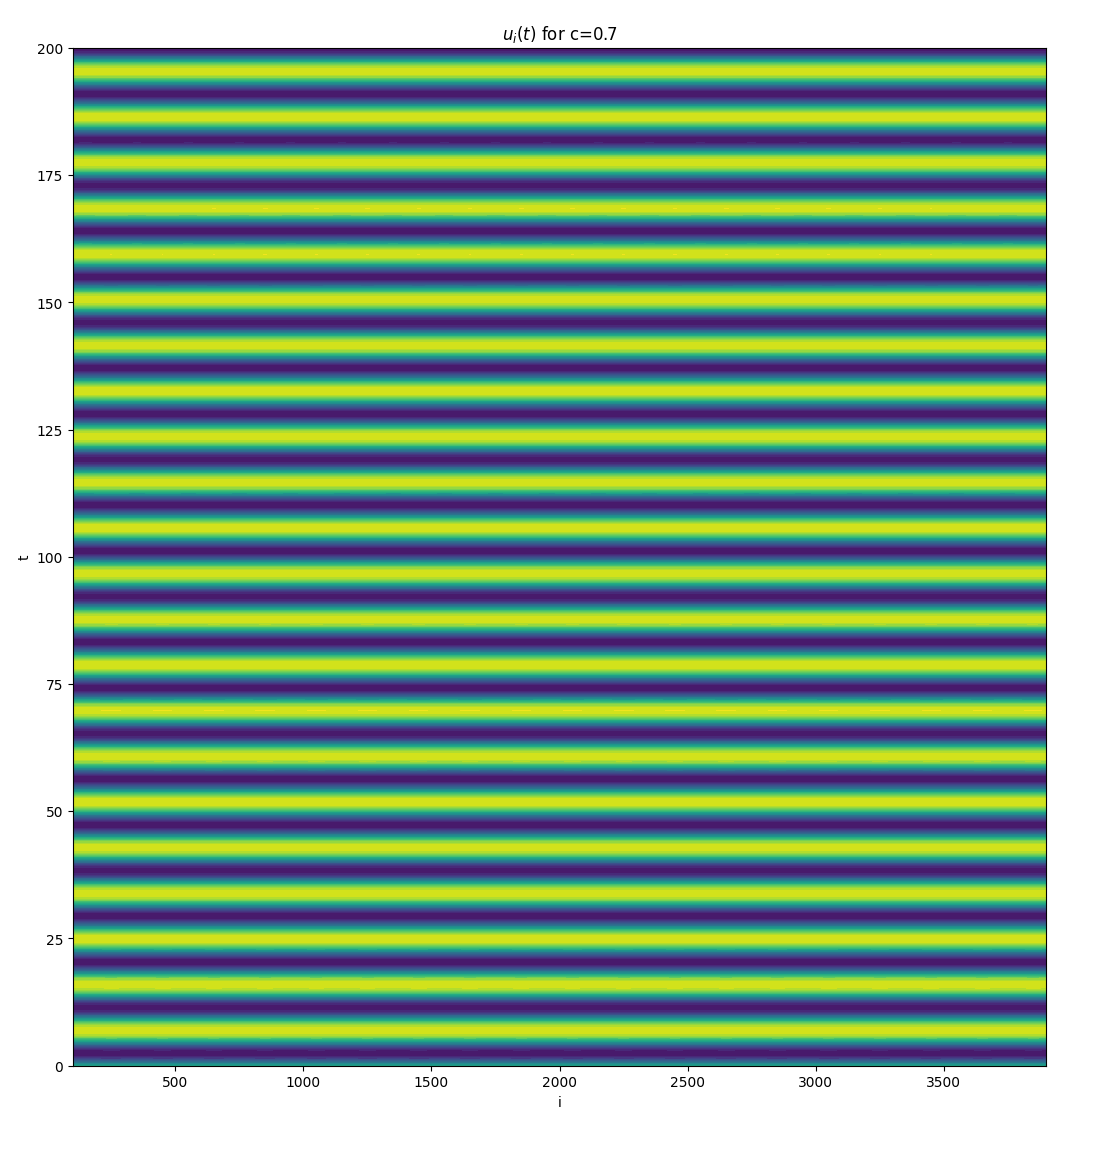
\includegraphics[width=0.6\textwidth]{./images/Pasted image 20231207115816.png}
    \caption{$u_i(t)$ for $c=0.7$}
\end{figure}

\begin{figure}[htpb]
    \centering
    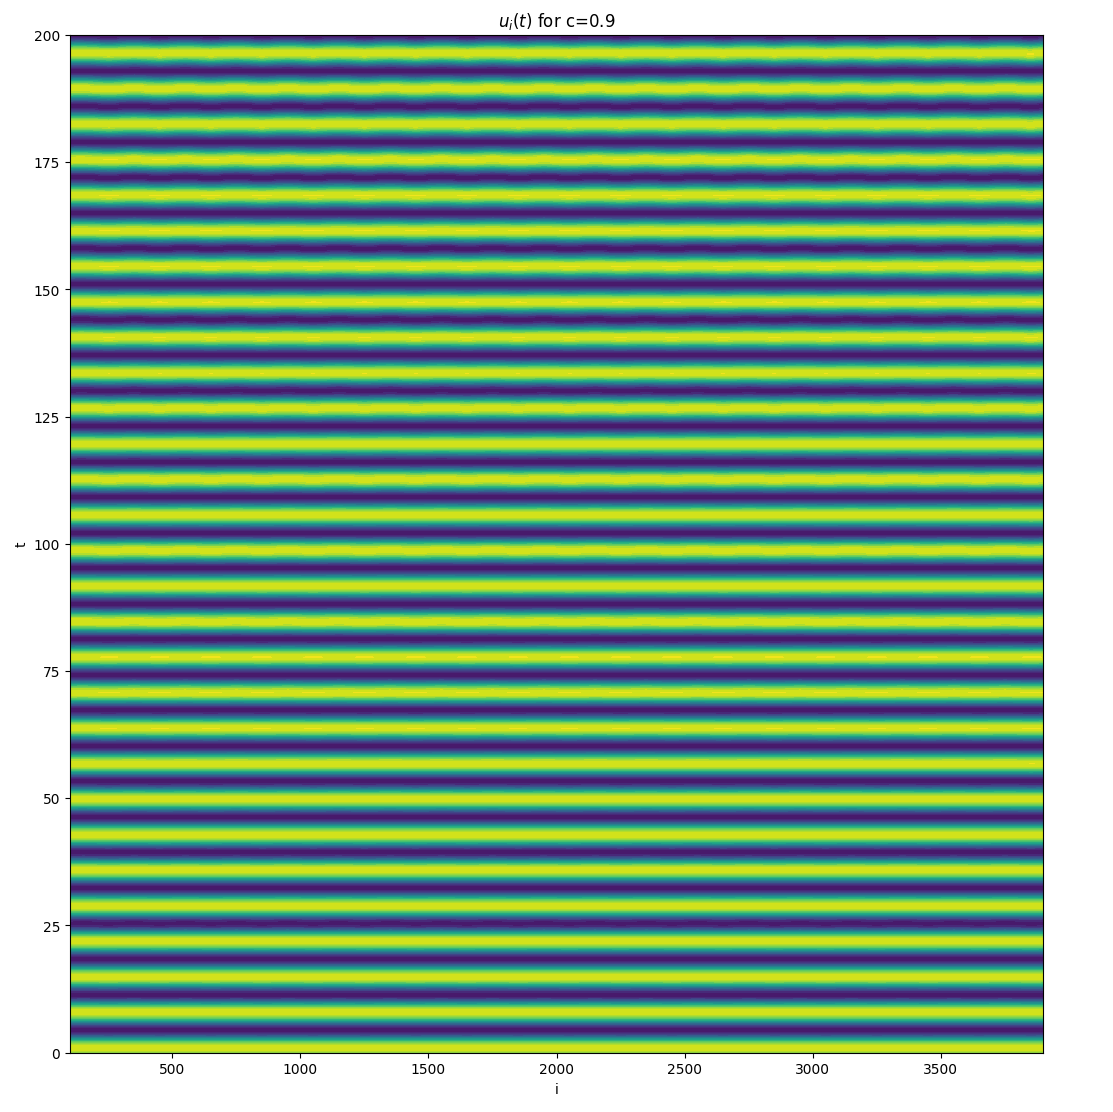
\includegraphics[width=0.6\textwidth]{./images/Pasted image 20231207115846.png}
    \caption{$u_i(t)$ for $c=0.5$}
\end{figure}

\begin{figure}[htpb]
    \centering
    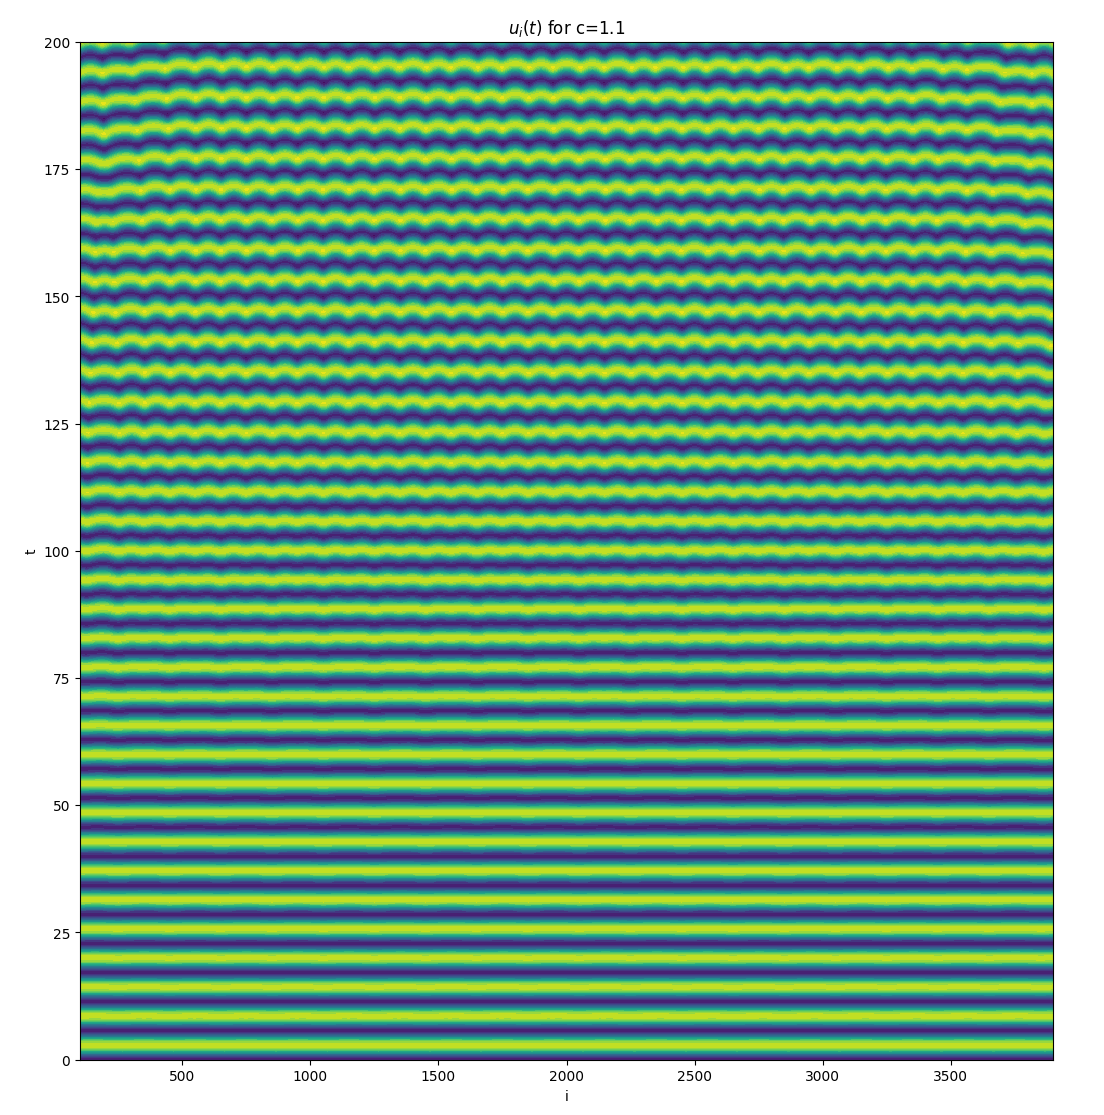
\includegraphics[width=0.6\textwidth]{./images/Pasted image 20231207115932.png}
    \caption{$u_i(t)$ for $c=1.1$}
\end{figure}

\begin{figure}[htpb]
    \centering
    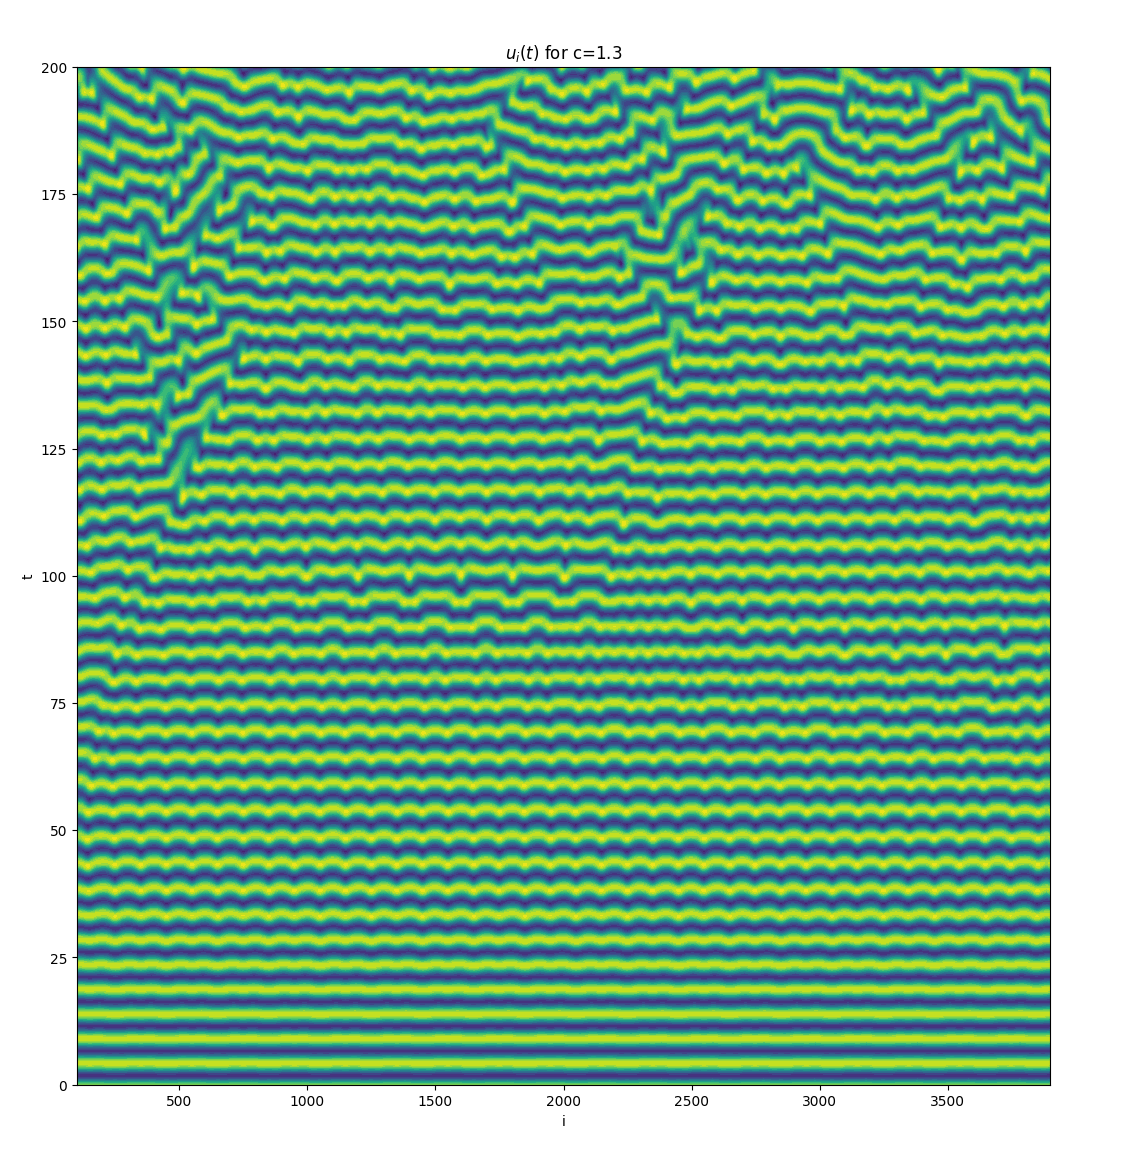
\includegraphics[width=0.6\textwidth]{./images/Pasted image 20231207120004.png}
    \caption{$u_i(t)$ for $c=1.3$}
\end{figure}

\begin{figure}[htpb]
    \centering
    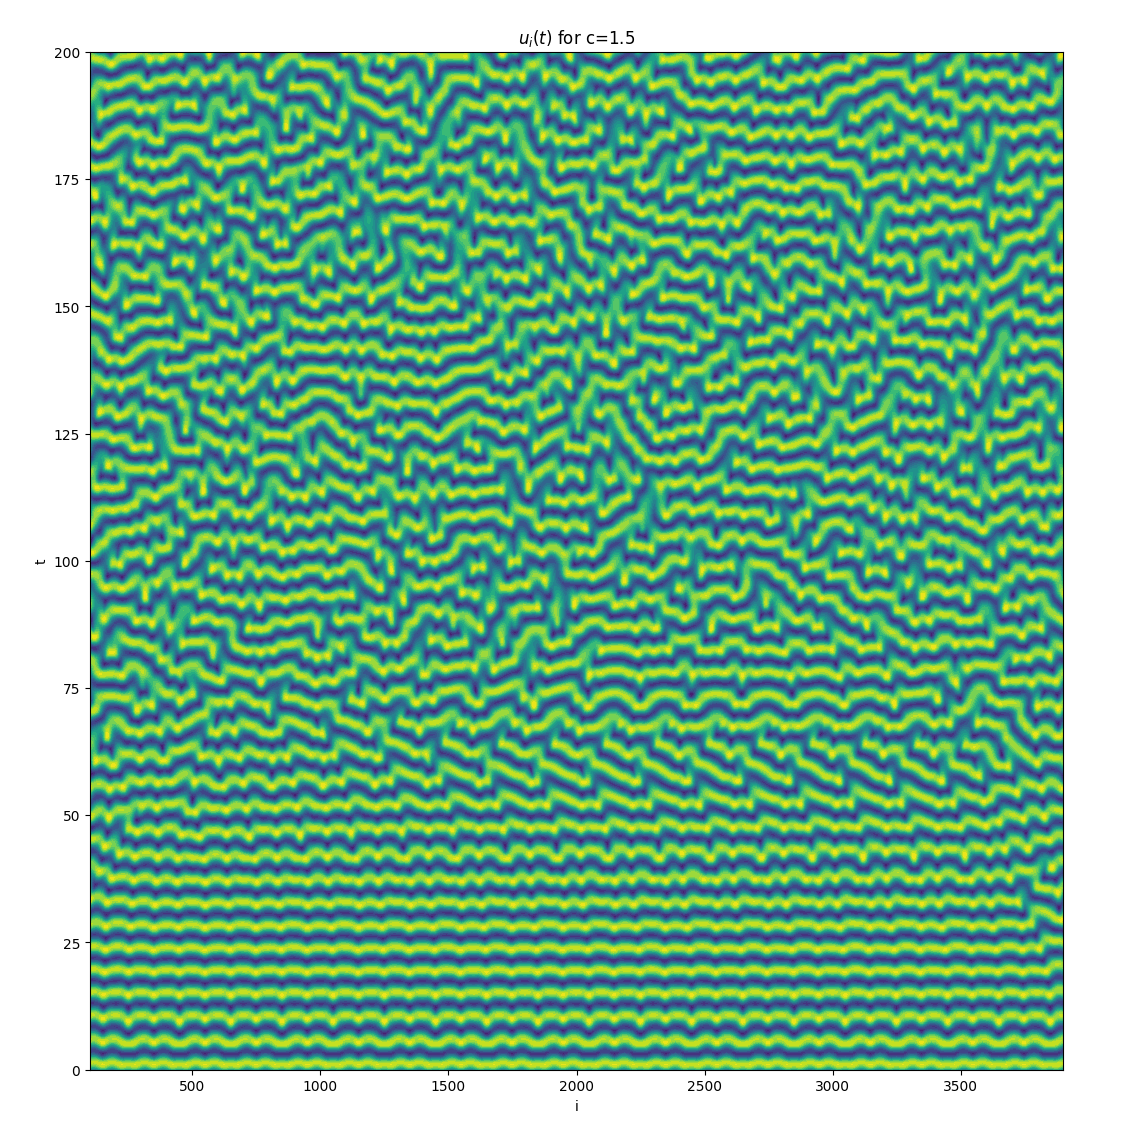
\includegraphics[width=1.0\textwidth]{./images/Pasted image 20231207120040.png}
    \caption{$u_i(t)$ for $c=1.5$}
\end{figure}

\clearpage

So now let us focus on the system when $c = 1.3$. As previously mentioned,
when $c=1.3$, we qualitatively observe regular steady sinusoidal behaviour for
$u(t)$  for small $t$, then as time progresses instabilities appear and the system becomes
more chaotic.

We again turn to PCA to examine the explained variances through time:

\begin{figure}[htpb]
    \centering
    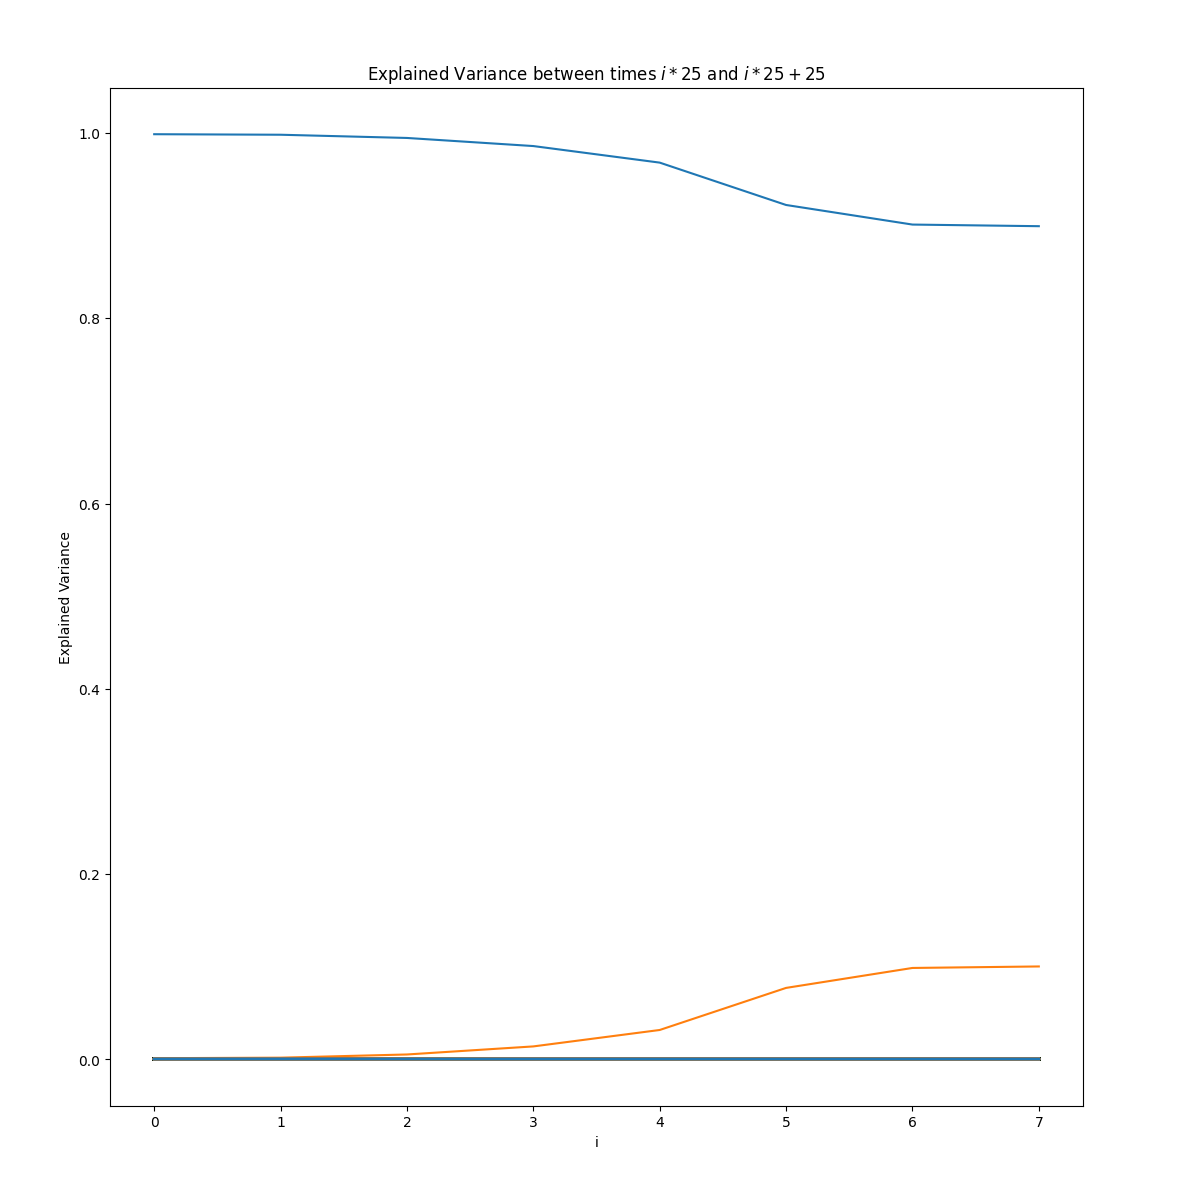
\includegraphics[width=1.0\textwidth]{./images/Pasted image 20231207142335.png}
    \caption{Explained variance attributed to each principal component. Different colors represent the variance explained by different principal components.}
\end{figure}

We calculate the percentage of variance explained by each principal component
in regular blocks of time. I.e we split the matrix $u$ into contiguous row intervals of length
25 and then apply PCA. Then the proportion of explained variance is given by:
$$
\frac{\lambda_{i}}{\sum \lambda _{j}}
$$
where $\lambda_{i}$ is the eigenvalue corresponding to the $i^{th}$ principal component.
We see that initially we can explain $100\%$ of the variance just using the first principal component.
This makes sense, since $u_{i}$ initially take the same values for fixed $t$. Then as we increase
$t$ we see that the explained variance due to 2nd principal component increases
and is no longer zero. The explained variance across all other components
remains zero. This shows us that for later times there are two main groups of solution
components which share similar within-group behaviour and within their groups
are correlated with each other and are not correlated to other components
in the opposing group. This evidences the divergent behaviour we qualitatively observed.


We next examine the correlation sum for $c=1.3$.
Since our data is highly auto-correlated in order to use the correlation sum to determine
the fractal dimension we need to use a time delay. For each component $u_i$, we use Welch's
method to determine the dominant frequency:

 \begin{figure}[htpb]
    \centering
    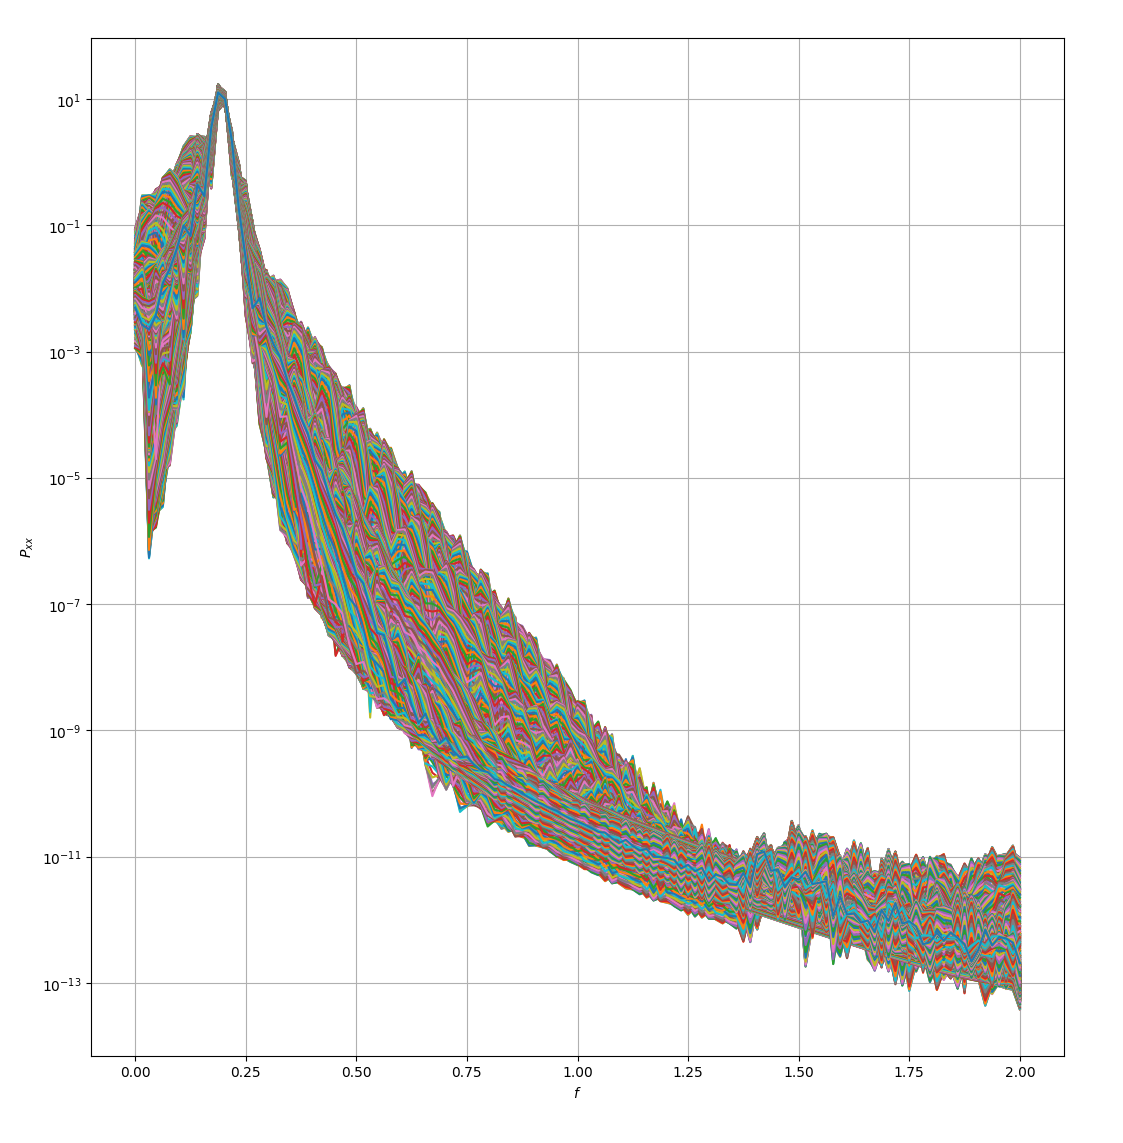
\includegraphics[width=1.0\textwidth]{./images/welches.png}
    \caption{Welch's method applied to $u_i$ for all $i$.}
\end{figure}
We observe that across all components we have the same dominant frequency, $f = 0.1875$.
We use this to set our time delay, $\tau := 1 / f$.

We account for the unwanted auto-correlation by only considering every
$\Delta := \left\lfloor \tau / \delta t \right\rfloor$ datapoint of $\bm{u}$.
Then using this filtered $\bm{u}$, we can calculate and plot the correlation sum: 


\begin{figure}[htpb]
    \centering
    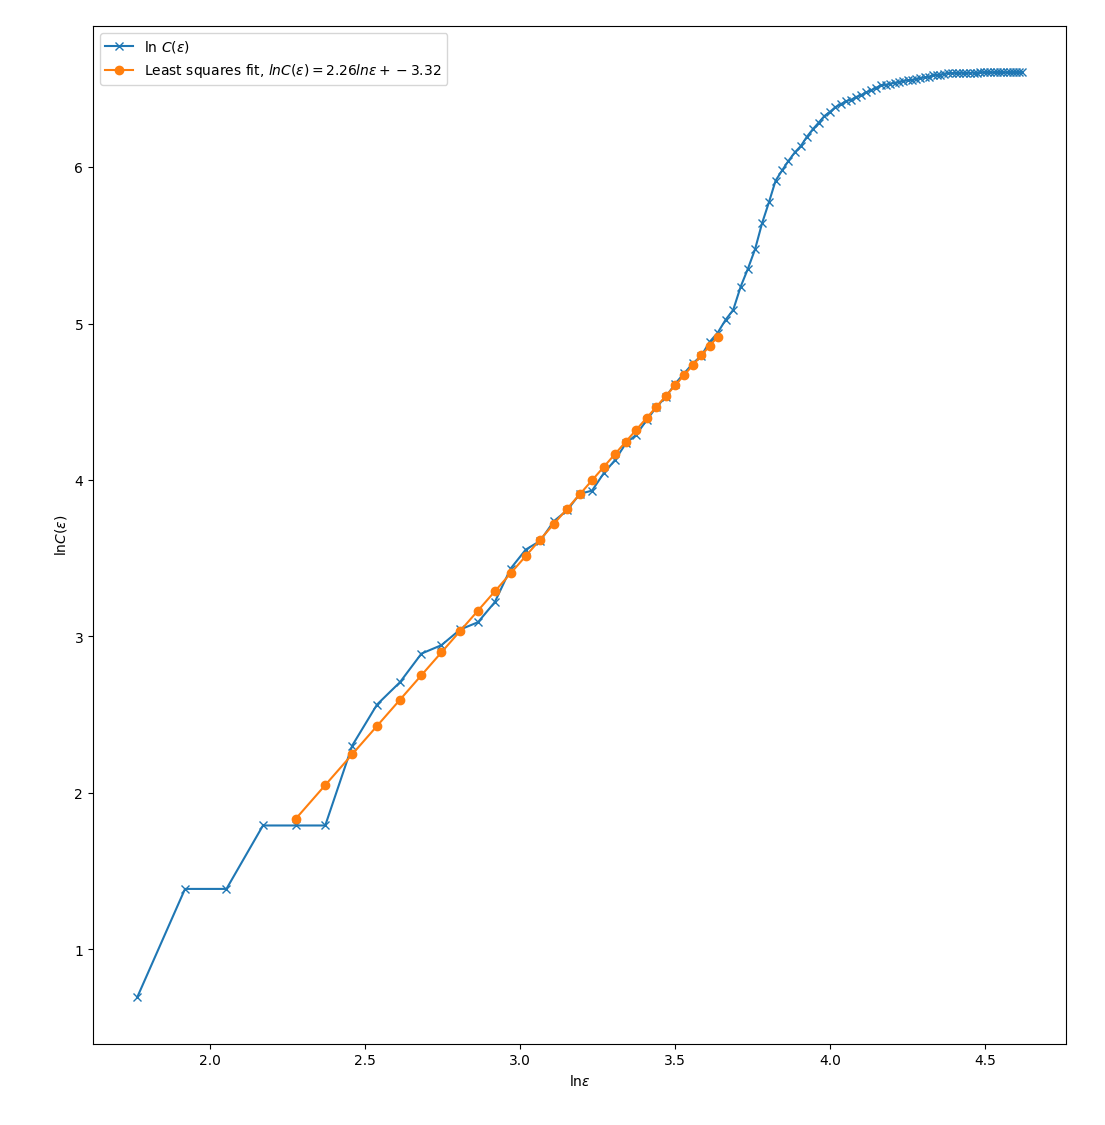
\includegraphics[width=1.0\textwidth]{./images/corr_sum.png}
    \caption{Estimating the fractal dimension $d$ using the regression  $\ln C(\epsilon) = d \ln \epsilon + c$}
\end{figure}

So we get a fractal dimension of $d \approx 2.26$. From lectures we know that for an autonomous system of ODEs, a dimension greater than $2$ is necessary for chaos and so our result
indicates weak/low-dimensional chaos. This agrees with what we qualitatively observed.


\subsection*{Part 3.2}
The code in part3q2 performs a low-rank approximation of the matrix A using its first $x$ principal components and then calculates the squared error between the original matrix and the reconstructed low rank approximation.

On the one hand one could argue that the code is efficient since we are taking advantage of the symmetry
of $A^T A$ by using np.linalg.eigh, which is much more efficient than using np.linalg.eig. However
we still have the expensive $A^T A$ calculation which we could avoid if instead we used np.linalg.svd
on $A$ directly.


% -----------------------------------------------------------------------
\end{document}
